\chapter{Structural  Mechanics   Model}
Static structural mechanics problems can be handled using the
class \code{StructuralMechanicsModel}.  So far, \akantu provides 2D and 3D
Bernoulli beam elements \cite{frey2009}.  This model is instantiated for a given
\code{Mesh}, as for the \code{SolidMechanicsModel}.  The model will create its own \code{FEEngine} object to
compute the interpolation, gradient, integration and assembly
operations.  The \code{StructuralMechanicsModel} constructor is called
in the following way:

\begin{cpp}
  StructuralMechanicsModel model(mesh, spatial_dimension);
\end{cpp}
where \code{mesh} is a \code{Mesh} object defining the structure for
which the equations of statics are to be solved, and
\code{spatial\_dimension} is the dimensionality of the problem.  If
\code{spatial\_dimension} is omitted, the problem is assumed to have
the same dimensionality as the one specified by the mesh.

\note[\ 1]{Dynamic computations are not supported to date.}

\note[\ 2]{Structural meshes are created and loaded as described in
  Section~\ref{sect:common:mesh} with \code{\_miot\_gmsh\_struct} instead  of \code{\_miot\_gmsh}:}

\begin{cpp}
  Mesh mesh;
  mesh.read("structural_mesh.msh", _miot_gmsh_struct);
\end{cpp}

This model contains at least the following \code{Arrays}:
\begin{description}
\item[blocked\_dofs] contains a Boolean value for each degree of
  freedom specifying whether that degree is blocked or not. A
  Dirichlet boundary condition can be prescribed by setting the
  \textbf{blocked\_dofs} value of a degree of freedom to
  \code{true}. The \textbf{displacement} is computed for all degrees
  of freedom for which the \textbf{blocked\_dofs} value is set to
  \code{false}. For the remaining degrees of freedom, the imposed
  values (zero by default after initialization) are kept.



\item[displacement\_rotation] contains the generalized displacements
  (\textit{i.e.} displacements and rotations) of all degrees of freedom. It can be
  either a computed displacement for free degrees of freedom or an
  imposed displacement in case of blocked ones ($\vec{u}$ in the
  following).

\item[external\_force] contains the generalized external forces (forces
  and moments) applied to the nodes ($\vec{f_{\st{ext}}}$ in the
  following).

\item[internal\_force] contains the generalized internal forces (forces
  and moments) applied to the nodes ($\vec{f_{\st{int}}}$ in the
  following).
\end{description}

An example to help understand how  to use this model will be presented in the
next section.

\section{Model Setup}
\label{sec:structMechMod:setup}

\subsection{Initialization}
The easiest way to initialize the structural mechanics model is:

\begin{cpp}
  model.initFull();
\end{cpp}
The method \code{initFull} computes the shape functions, initializes
the internal vectors mentioned above and allocates the memory for the
stiffness matrix, unlike the solid mechanics model, its default argument is \code{\_static}.

Material properties are defined using the \code{StructuralMaterial}
structure described in
Table~\ref{tab:structMechMod:strucMaterial}. Such a definition could,
for instance, look like
\begin{cpp}
  StructuralMaterial mat1;
  mat.E=3e10;
  mat.I=0.0025;
  mat.A=0.01;
\end{cpp}

\begin{table}[htb] \centering
  \begin{tabular}{cl}
    \toprule
    Field  & Description \\
    \midrule
    \code{E} & Young's  modulus  \\
    \code{A}  & Cross  section  area  \\
    \code{I} & Second cross sectional  moment of inertia (for 2D elements)\\
    \code{Iy} & \code{I}  around beam $y$--axis (for 3D elements)\\
    \code{Iz} & \code{I}  around beam $z$--axis (for 3D elements)\\
    \code{GJ}  & Polar  moment of inertia  of beam  cross section (for 3D elements)\\
    \bottomrule
  \end{tabular}
  \caption{Material properties  for structural elements  defined in
the class \code{StructuralMaterial}.}
  \label{tab:structMechMod:strucMaterial}
\end{table}
Materials can be added to the model's \code{element\_material} vector using
\begin{cpp}
  model.addMaterial(mat1);
\end{cpp}

They are successively numbered and then assigned to specific elements.
\begin{cpp}
for (UInt i = 0; i < nb_element_mat_1; ++i) {
    model.getElementMaterial(_bernoulli_beam_2)(i,0) = 1;
  }
\end{cpp}


\subsection{Setting Boundary Conditions}\label{sect:structMechMod:boundary}

As explained before, the Dirichlet boundary conditions are applied through the
array \textbf{blocked\_dofs}. Two options exist to define Neumann conditions.
If a nodal force is applied, it has to be directly set in the array
\textbf{force\_momentum}. For loads distributed along the beam length, the
method \code{computeForcesFromFunction} integrates them into nodal forces.  The
method takes as input a function describing the distribution of loads along the
beam and a functor \code{BoundaryFunctionType} specifing if the function is
expressed in the local coordinates (\code{\_bft\_traction\_local}) or in the
global system of coordinates (\code{\_bft\_traction}).
\begin{cpp}
 static void lin_load(double * position, double * load,
		      Real * normal, UInt surface_id){
  memset(load,0,sizeof(Real)*3);
  load[1] = position[0]*position[0]-250;
}
int main(int argc, char *argv[]){
...
model.computeForcesFromFunction<_bernoulli_beam_2>(lin_load,
                                                   _bft_traction_local);
...}
\end{cpp}


\section{Static Analysis\label{sect:structMechMod:static}}

The \code{StructuralMechanicsModel} class can perform static analyses
of structures.  In this case, the equation to solve is the same as for
the \code{SolidMechanicsModel} used for static analyses
\begin{equation}\label{eqn:structMechMod:static}
  \mat{K} \vec{u} = \vec{f_{\st{ext}}}~,
\end{equation}
where $\mat{K}$ is the global stiffness matrix, $\vec{u}$ the
generalized displacement vector and $\vec{f_{\st{ext}}}$ the vector of
generalized external forces applied to the system.

To solve such a problem, the static solver of the
\code{StructuralMechanicsModel}\index{StructuralMechanicsModel} object
is used.  First a model has to be created and initialized.

\begin{cpp}
  StructuralMechanicsModel model(mesh);
  model.initFull();
\end{cpp}


\begin{itemize}
\item \code{model.initFull} initializes all internal vectors to zero.
\end{itemize}


Once the model is created and initialized, the boundary conditions can
be set as explained in Section~\ref{sect:structMechMod:boundary}.
Boundary conditions will prescribe the external forces or moments for
the free degrees of freedom $\vec{f_{\st{ext}}}$ and displacements or
rotations for the others.  To completely define the system represented
by equation (\ref{eqn:structMechMod:static}), the global stiffness
matrix $\mat{K}$ must be assembled.
\index{StructuralMechanicsModel!assembleStiffnessMatrix}

\begin{cpp}
  model.assembleStiffnessMatrix();
\end{cpp}

The computation of the static equilibrium is performed using the same
Newton-Raphson algorithm as described in
Section~\ref{sect:smm:static}.

\note{To date,
\code{StructuralMechanicsModel} handles only constitutively and
geometrically linear problems, the algorithm is therefore guaranteed
to converge in two iterations.}

\begin{cpp}
  model.updateResidual();
  model.solve();
\end{cpp}
\index{StructuralMechanicsModel!updateResidual}
\index{StructuralMechanicsModel!solve}

\begin{itemize}

\item \code{model.updateResidual} assembles the internal forces and
  removes them from the external forces.
\item \code{model.solve} solves the Equation (\ref{eqn:structMechMod:static}).
  The \textbf{increment} vector of the model will contain the new
  increment of displacements, and the \textbf{displacement\_rotation}
  vector is also updated to the new displacements.

\end{itemize}

%At the end of the analysis, the final solution is stored in the
%\textbf{displacement} vector.  A full example of how to solve a
%structural mechanics problem is presented in the code
%\shellcode{\examplesdir/structural\_mechanics/test\_structural\_mechanics\_model\_bernoulli\_beam\_2\_exemple\_1\_1.cc}.
%This example is composed of a 2D beam, clamped at the left end and
%supported by two rollers as shown in Figure
%\ref{fig:structMechMod:exem1_1}.  The problem is defined by the
%applied load $q=\SI{6}{\kilo\newton\per\metre}$, moment $\bar{M} =
%\SI{3.6}{\kilo\newton\metre}$, moments of inertia $I_1 =
%\SI{250\,000}{\power{\centi\metre}{4}}$ and $I_2 =
%\SI{128\,000}{\power{\centi\metre}{4}}$ and lengths $L_1 =
%\SI{10}{\metre}$ and $L_2 = \SI{8}{\metre}$.  The resulting
%rotations at node two and three are $ \varphi_2 = 0.001\,167\
%\mbox{and}\ \varphi_3 = -0.000\,771.$

At the end of the analysis, the final solution is stored in the
\textbf{displacement\_rotation} vector.  A full example of how to
solve a structural mechanics problem is presented in the code
\shellcode{\examplesdir/structural\_mechanics/bernoulli\_beam\_2\_example.cc}.
This example is composed of a 2D beam, clamped at the left end and
supported by two rollers as shown in Figure
\ref{fig:structMechMod:exem1_1}.  The problem is defined by the
applied load $q=\SI{6}{\kilo\newton\per\metre}$, moment $\bar{M} =
\SI{3.6}{\kilo\newton\metre}$, moments of inertia $I_1 =
\SI{250\,000}{\centi\metre\tothe{4}}$ and $I_2 =
\SI{128\,000}{\centi\metre\tothe{4}}$ and lengths $L_1 =
\SI{10}{\metre}$ and $L_2 = \SI{8}{\metre}$.  The resulting
rotations at node two and three are $ \varphi_2 = 0.001\,167\
\mbox{and}\ \varphi_3 = -0.000\,771.$

 \begin{figure}[htb]
   \centering
   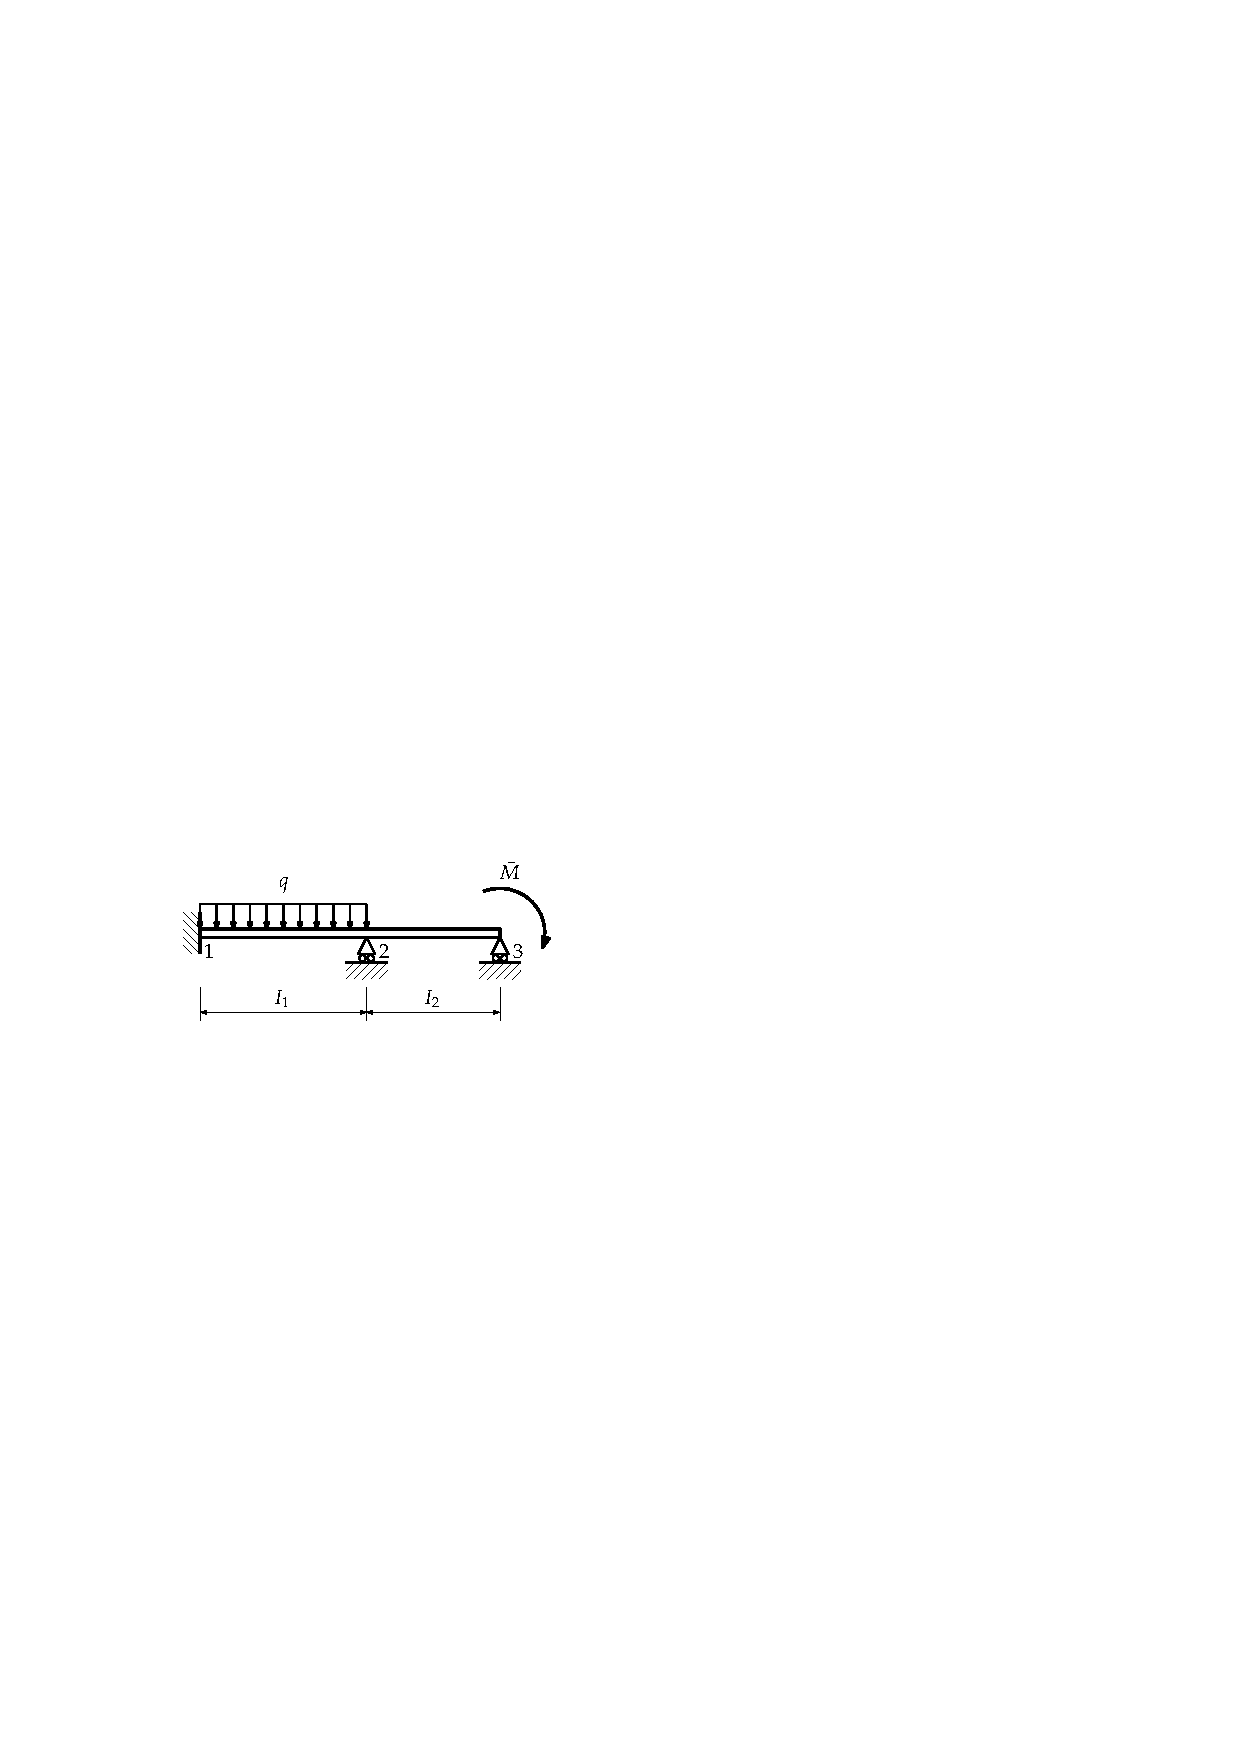
\includegraphics[scale=1.1]{figures/beam_example}
   \caption{2D beam example}
   \label{fig:structMechMod:exem1_1}
 \end{figure}





%%% Local Variables:
%%% mode: latex
%%% TeX-master: "manual"
%%% End:
